\documentclass{standalone}
\usepackage{tikz}
\usetikzlibrary{patterns, positioning}

\begin{document}
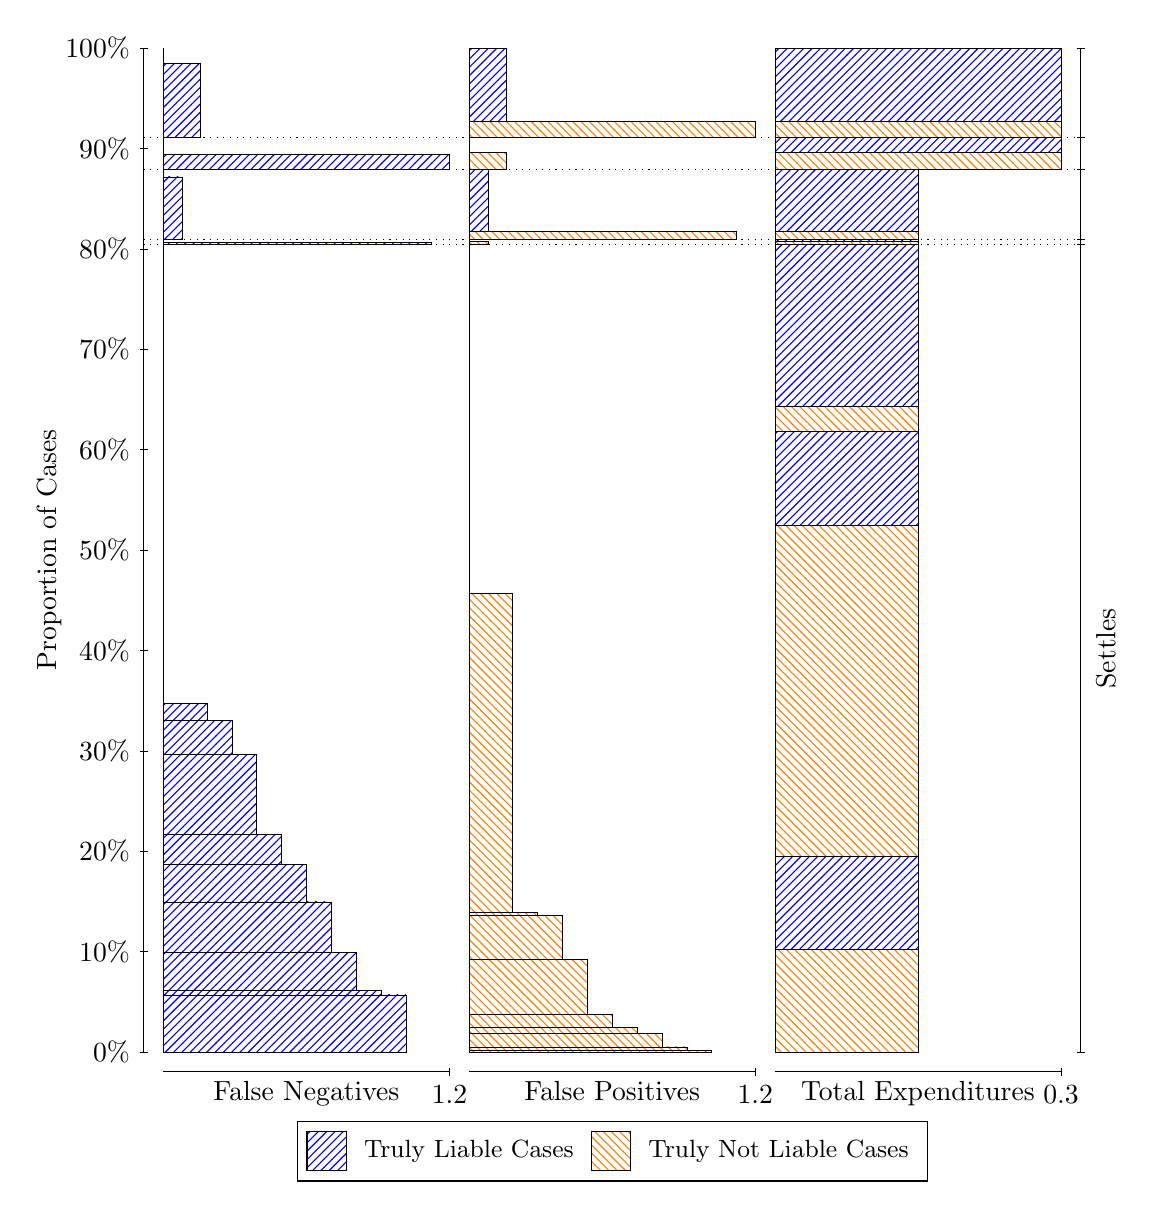
\begin{tikzpicture}
\draw[black, very thin] (1.5,1.75) -- (1.5,14.5);
\node[rotate=90, anchor=center] at (0.3, 8.125) {Proportion of Cases};
\draw[black, very thin] (1.45,1.75) -- (1.55,1.75);
\node[anchor=east] at (1.45, 1.75) {0\%};
\draw[black, very thin] (1.45,3.025) -- (1.55,3.025);
\node[anchor=east] at (1.45, 3.025) {10\%};
\draw[black, very thin] (1.45,4.3) -- (1.55,4.3);
\node[anchor=east] at (1.45, 4.3) {20\%};
\draw[black, very thin] (1.45,5.575) -- (1.55,5.575);
\node[anchor=east] at (1.45, 5.575) {30\%};
\draw[black, very thin] (1.45,6.85) -- (1.55,6.85);
\node[anchor=east] at (1.45, 6.85) {40\%};
\draw[black, very thin] (1.45,8.125) -- (1.55,8.125);
\node[anchor=east] at (1.45, 8.125) {50\%};
\draw[black, very thin] (1.45,9.4) -- (1.55,9.4);
\node[anchor=east] at (1.45, 9.4) {60\%};
\draw[black, very thin] (1.45,10.675) -- (1.55,10.675);
\node[anchor=east] at (1.45, 10.675) {70\%};
\draw[black, very thin] (1.45,11.95) -- (1.55,11.95);
\node[anchor=east] at (1.45, 11.95) {80\%};
\draw[black, very thin] (1.45,13.225) -- (1.55,13.225);
\node[anchor=east] at (1.45, 13.225) {90\%};
\draw[black, very thin] (1.45,14.5) -- (1.55,14.5);
\node[anchor=east] at (1.45, 14.5) {100\%};

\draw[black, very thin] (13.4,1.75) -- (13.4,14.5);
\draw[black, very thin] (13.35,1.75) -- (13.45,1.75);
\node[anchor=west] at (13.35, 1.75) {};
\draw[black, very thin] (13.35,12.002) -- (13.45,12.002);
\node[anchor=west] at (13.35, 12.002) {};
\draw[black, very thin] (13.35,12.074) -- (13.45,12.074);
\node[anchor=west] at (13.35, 12.074) {};
\draw[black, very thin] (13.35,12.959) -- (13.45,12.959);
\node[anchor=west] at (13.35, 12.959) {};
\draw[black, very thin] (13.35,13.369) -- (13.45,13.369);
\node[anchor=west] at (13.35, 13.369) {};
\draw[black, very thin] (13.35,14.5) -- (13.45,14.5);
\node[anchor=west] at (13.35, 14.5) {};

\draw[black, very thin, pattern color=blue, pattern=north east lines] (1.75,1.75) rectangle (4.8304,2.4753);
\draw[black, very thin, pattern color=blue, pattern=north east lines] (1.75,2.4753) rectangle (4.5145,2.5328);
\draw[black, very thin, pattern color=blue, pattern=north east lines] (1.75,2.5328) rectangle (4.1986,3.015);
\draw[black, very thin, pattern color=blue, pattern=north east lines] (1.75,3.015) rectangle (3.8826,3.655);
\draw[black, very thin, pattern color=blue, pattern=north east lines] (1.75,3.655) rectangle (3.5667,4.1287);
\draw[black, very thin, pattern color=blue, pattern=north east lines] (1.75,4.1287) rectangle (3.2507,4.5107);
\draw[black, very thin, pattern color=blue, pattern=north east lines] (1.75,4.5107) rectangle (2.9348,5.534);
\draw[black, very thin, pattern color=blue, pattern=north east lines] (1.75,5.534) rectangle (2.6188,5.9611);
\draw[black, very thin, pattern color=blue, pattern=north east lines] (1.75,5.9611) rectangle (2.3029,6.1804);
\draw[black, very thin, pattern color=orange, pattern=north west lines] (1.75,6.1804) rectangle (1.75,12.002);
\draw[black, very thin, pattern color=blue, pattern=north east lines] (1.75,12.002) rectangle (5.1464,12.029);
\draw[black, very thin, pattern color=orange, pattern=north west lines] (1.75,12.029) rectangle (1.75,12.074);
\draw[black, very thin, pattern color=blue, pattern=north east lines] (1.75,12.074) rectangle (1.987,12.864);
\draw[black, very thin, pattern color=orange, pattern=north west lines] (1.75,12.864) rectangle (1.75,12.959);
\draw[black, very thin, pattern color=blue, pattern=north east lines] (1.75,12.959) rectangle (5.3833,13.152);
\draw[black, very thin, pattern color=orange, pattern=north west lines] (1.75,13.152) rectangle (1.75,13.369);
\draw[black, very thin, pattern color=blue, pattern=north east lines] (1.75,13.369) rectangle (2.2239,14.304);
\draw[black, very thin, pattern color=orange, pattern=north west lines] (1.75,14.304) rectangle (1.75,14.5);
\draw[black, very thin, pattern color=orange, pattern=north west lines] (5.6333,1.75) rectangle (8.7138,1.7699);
\draw[black, very thin, pattern color=orange, pattern=north west lines] (5.6333,1.7699) rectangle (8.3978,1.8155);
\draw[black, very thin, pattern color=orange, pattern=north west lines] (5.6333,1.8155) rectangle (8.0819,1.9824);
\draw[black, very thin, pattern color=orange, pattern=north west lines] (5.6333,1.9824) rectangle (7.7659,2.0654);
\draw[black, very thin, pattern color=orange, pattern=north west lines] (5.6333,2.0654) rectangle (7.45,2.2229);
\draw[black, very thin, pattern color=orange, pattern=north west lines] (5.6333,2.2229) rectangle (7.1341,2.2256);
\draw[black, very thin, pattern color=orange, pattern=north west lines] (5.6333,2.2256) rectangle (7.1341,2.9242);
\draw[black, very thin, pattern color=orange, pattern=north west lines] (5.6333,2.9242) rectangle (6.8181,3.4893);
\draw[black, very thin, pattern color=orange, pattern=north west lines] (5.6333,3.4893) rectangle (6.5022,3.5232);
\draw[black, very thin, pattern color=orange, pattern=north west lines] (5.6333,3.5232) rectangle (6.1862,7.5716);
\draw[black, very thin, pattern color=blue, pattern=north east lines] (5.6333,7.5716) rectangle (5.6333,12.002);
\draw[black, very thin, pattern color=orange, pattern=north west lines] (5.6333,12.002) rectangle (5.8703,12.047);
\draw[black, very thin, pattern color=blue, pattern=north east lines] (5.6333,12.047) rectangle (5.6333,12.074);
\draw[black, very thin, pattern color=orange, pattern=north west lines] (5.6333,12.074) rectangle (9.0297,12.17);
\draw[black, very thin, pattern color=blue, pattern=north east lines] (5.6333,12.17) rectangle (5.8703,12.959);
\draw[black, very thin, pattern color=orange, pattern=north west lines] (5.6333,12.959) rectangle (6.1072,13.176);
\draw[black, very thin, pattern color=blue, pattern=north east lines] (5.6333,13.176) rectangle (5.6333,13.369);
\draw[black, very thin, pattern color=orange, pattern=north west lines] (5.6333,13.369) rectangle (9.2667,13.565);
\draw[black, very thin, pattern color=blue, pattern=north east lines] (5.6333,13.565) rectangle (6.1072,14.5);
\draw[black, very thin, pattern color=orange, pattern=north west lines] (9.5167,1.75) rectangle (11.333,3.0503);
\draw[black, very thin, pattern color=blue, pattern=north east lines] (9.5167,3.0503) rectangle (11.333,4.2301);
\draw[black, very thin, pattern color=orange, pattern=north west lines] (9.5167,4.2301) rectangle (11.333,8.436);
\draw[black, very thin, pattern color=blue, pattern=north east lines] (9.5167,8.436) rectangle (11.333,9.6349);
\draw[black, very thin, pattern color=orange, pattern=north west lines] (9.5167,9.6349) rectangle (11.333,9.9503);
\draw[black, very thin, pattern color=blue, pattern=north east lines] (9.5167,9.9503) rectangle (11.333,12.002);
\draw[black, very thin, pattern color=orange, pattern=north west lines] (9.5167,12.002) rectangle (11.333,12.047);
\draw[black, very thin, pattern color=blue, pattern=north east lines] (9.5167,12.047) rectangle (11.333,12.074);
\draw[black, very thin, pattern color=orange, pattern=north west lines] (9.5167,12.074) rectangle (11.333,12.17);
\draw[black, very thin, pattern color=blue, pattern=north east lines] (9.5167,12.17) rectangle (11.333,12.959);
\draw[black, very thin, pattern color=orange, pattern=north west lines] (9.5167,12.959) rectangle (13.15,13.176);
\draw[black, very thin, pattern color=blue, pattern=north east lines] (9.5167,13.176) rectangle (13.15,13.369);
\draw[black, very thin, pattern color=orange, pattern=north west lines] (9.5167,13.369) rectangle (13.15,13.565);
\draw[black, very thin, pattern color=blue, pattern=north east lines] (9.5167,13.565) rectangle (13.15,14.5);
\draw[black, dotted] (1.5,12.002) -- (13.4,12.002);
\draw[black, dotted] (1.5,12.074) -- (13.4,12.074);
\draw[black, dotted] (1.5,12.959) -- (13.4,12.959);
\draw[black, dotted] (1.5,13.369) -- (13.4,13.369);
\draw[black, very thin] (1.75,1.5) -- (5.3833,1.5);
\node[anchor=north] at (3.5667, 1.5) {False Negatives};
\draw[black, very thin] (5.3833,1.45) -- (5.3833,1.55);
\node[anchor=north] at (5.3833, 1.45) {1.2};

\draw[black, very thin] (5.6333,1.5) -- (9.2667,1.5);
\node[anchor=north] at (7.45, 1.5) {False Positives};
\draw[black, very thin] (9.2667,1.45) -- (9.2667,1.55);
\node[anchor=north] at (9.2667, 1.45) {1.2};

\draw[black, very thin] (9.5167,1.5) -- (13.15,1.5);
\node[anchor=north] at (11.333, 1.5) {Total Expenditures};
\draw[black, very thin] (13.15,1.45) -- (13.15,1.55);
\node[anchor=north] at (13.15, 1.45) {0.3};

\node[black, centered, rotate=90] at (13.72, 6.876) {Settles};





\draw (7.449999999999999,1.5) node[draw=none] (baseCoordinate) {};
\begin{scope}[align=center]
        \matrix[scale=0.5, draw=black, below=0.5cm of baseCoordinate, nodes={draw}, column sep=0.1cm]{
            \node[rectangle, draw, minimum width=0.5cm, minimum height=0.5cm, pattern=north east lines, pattern color=blue] {}; &
            \node[draw=none, font=\small] (B) {Truly Liable Cases}; &
            \node[rectangle, draw, minimum width=0.5cm, minimum height=0.5cm, pattern=north west lines, pattern color=orange] {}; &
            \node[draw=none, font=\small] (B) {Truly Not Liable Cases}; \\
            };
\end{scope}

\end{tikzpicture}
\end{document}